
\documentclass[12pt]{article}
\usepackage[english]{babel}
\usepackage[T1]{fontenc}
\usepackage[utf8]{inputenc}
\usepackage{delarray,amsmath,bbm,epsfig,slashed}
\newcommand{\pat}{\partial}
\newcommand{\be}{\begin{equation}}
\newcommand{\ee}{\end{equation}}
\newcommand{\bea}{\begin{eqnarray}}
\newcommand{\eea}{\end{eqnarray}}
\newcommand{\abf}{{\bf a}}
\newcommand{\Zmath}{\mathbf{Z}}
\newcommand{\Zcal}{{\cal Z}_{12}}
\newcommand{\zcal}{z_{12}}
\newcommand{\Acal}{{\cal A}}
\newcommand{\Fcal}{{\cal F}}
\newcommand{\Ucal}{{\cal U}}
\newcommand{\Vcal}{{\cal V}}
\newcommand{\Ocal}{{\cal O}}
\newcommand{\Rcal}{{\cal R}}
\newcommand{\Scal}{{\cal S}}
\newcommand{\Lcal}{{\cal L}}
\newcommand{\Hcal}{{\cal H}}
\newcommand{\hsf}{{\sf h}}
\newcommand{\half}{\frac{1}{2}}
\newcommand{\Xbar}{\bar{X}}
\newcommand{\xibar}{\bar{\xi }}
\newcommand{\barh}{\bar{h}}
\newcommand{\Ubar}{\bar{\cal U}}
\newcommand{\Vbar}{\bar{\cal V}}
\newcommand{\Fbar}{\bar{F}}
\newcommand{\zbar}{\bar{z}}
\newcommand{\wbar}{\bar{w}}
\newcommand{\zbarhat}{\hat{\bar{z}}}
\newcommand{\wbarhat}{\hat{\bar{w}}}
\newcommand{\wbartilde}{\tilde{\bar{w}}}
\newcommand{\barone}{\bar{1}}
\newcommand{\bartwo}{\bar{2}}
\newcommand{\nbyn}{N \times N}
\newcommand{\repres}{\leftrightarrow}
\newcommand{\Tr}{{\rm Tr}}
\newcommand{\tr}{{\rm tr}}
\newcommand{\ninfty}{N \rightarrow \infty}
\newcommand{\unitk}{{\bf 1}_k}
\newcommand{\unitm}{{\bf 1}}
\newcommand{\zerom}{{\bf 0}}
\newcommand{\unittwo}{{\bf 1}_2}
\newcommand{\holo}{{\cal U}}
%\newcommand{\bra}{\langle}
%\newcommand{\ket}{\rangle}
\newcommand{\muhat}{\hat{\mu}}
\newcommand{\nuhat}{\hat{\nu}}
\newcommand{\rhat}{\hat{r}}
\newcommand{\phat}{\hat{\phi}}
\newcommand{\that}{\hat{t}}
\newcommand{\shat}{\hat{s}}
\newcommand{\zhat}{\hat{z}}
\newcommand{\what}{\hat{w}}
\newcommand{\sgamma}{\sqrt{\gamma}}
\newcommand{\bfE}{{\bf E}}
\newcommand{\bfB}{{\bf B}}
\newcommand{\bfM}{{\bf M}}
\newcommand{\cl} {\cal l}
\newcommand{\ctilde}{\tilde{\chi}}
\newcommand{\ttilde}{\tilde{t}}
\newcommand{\ptilde}{\tilde{\phi}}
\newcommand{\utilde}{\tilde{u}}
\newcommand{\vtilde}{\tilde{v}}
\newcommand{\wtilde}{\tilde{w}}
\newcommand{\ztilde}{\tilde{z}}

% David Weir's macros


\newcommand{\nn}{\nonumber}
\newcommand{\com}[2]{\left[{#1},{#2}\right]}
\newcommand{\mrm}[1] {{\mathrm{#1}}}
\newcommand{\mbf}[1] {{\mathbf{#1}}}
\newcommand{\ave}[1]{\left\langle{#1}\right\rangle}
\newcommand{\halft}{{\textstyle \frac{1}{2}}}
\newcommand{\ie}{{\it i.e.\ }}
\newcommand{\eg}{{\it e.g.\ }}
\newcommand{\cf}{{\it cf.\ }}
\newcommand{\etal}{{\it et al.}}
\newcommand{\ket}[1]{\vert{#1}\rangle}
\newcommand{\bra}[1]{\langle{#1}\vert}
\newcommand{\bs}[1]{\boldsymbol{#1}}
\newcommand{\xv}{{\bs{x}}}
\newcommand{\yv}{{\bs{y}}}
\newcommand{\pv}{{\bs{p}}}
\newcommand{\kv}{{\bs{k}}}
\newcommand{\qv}{{\bs{q}}}
\newcommand{\bv}{{\bs{b}}}
\newcommand{\ev}{{\bs{e}}}
\newcommand{\gv}{\bs{\gamma}}
\newcommand{\lv}{{\bs{\ell}}}
\newcommand{\nabv}{{\bs{\nabla}}}
\newcommand{\sigv}{{\bs{\sigma}}}
\newcommand{\notvec}{\bs{0}_\perp}
\newcommand{\inv}[1]{\frac{1}{#1}}
%\newcommand{\xv}{{\bs{x}}}
%\newcommand{\yv}{{\bs{y}}}
\newcommand{\Av}{\bs{A}}
%\newcommand{\lv}{{\bs{\ell}}}

%\newcommand\bsigma{\vec{\sigma}}
\hoffset 0.5cm
\voffset -0.4cm
\evensidemargin -0.2in
\oddsidemargin -0.2in
\topmargin -0.2in
\textwidth 6.3in
\textheight 8.4in

\begin{document}

\normalsize

\baselineskip 14pt

\begin{center}
{\Large {\bf Quantum Information A \ \ Fall 2020 \ \  Exam Solutions}}\\
{\large { Jake Muff}}\\
{Student number: 015361763}\\
{21/10/2020}
\end{center}


%Problems 3 and 4 are from J. J. Sakurai: {\em Modern Quantum Mechanics}, numbers 3.2 and 3.8, respectively.

\begin{enumerate}

\item \textbf{\underline{Exercise 3.29 from Nielsen \& Chuang.}}
\\
Show that applying two consecutive Fredkin gates gives the same output as input. (Fredkin gate is self inverse)
\\
Fredkin gate only swaps bits or leaves them alone so number of 1's or 0's in the output must be the same as input i.e 
$$ (x,y,z) \rightarrow (x,xz+\tilde{x}y, xy + \tilde{x}z)$$
So the only thing that changes the output is the control bit $c$ which, for two consecutive inputs as 4 different permutations
\begin{table}[h]
    \centering
    \begin{tabular}{|c|c|}
    \hline
    \multicolumn{2}{|c|}{c} \\ \hline
    0          & 0          \\ \hline
    0          & 1          \\ \hline
    1          & 0          \\ \hline
    1          & 1          \\ \hline
    \end{tabular}
    \caption{Table showing that different permutations or values the control bit can be with two consecutive Fredkin gates. }
    \label{tab1}
    \end{table}
    \begin{table}[h!]
        \centering
        \begin{tabular}{ccl}
        a & $\rightarrow$ & a' \\
        b & $\rightarrow$ & b' \\
        c & $\rightarrow$ & c'
        \end{tabular}
        \begin{tabular}{ccl}
            a & $\rightarrow$ & b' \\
            b & $\rightarrow$ & a' \\
            c & $\rightarrow$ & c'
            \end{tabular}
        \caption{If c=0(left) and c=1(right), for 1 Fredkin gate.}
        \label{tab1}
        \end{table}
    
        \begin{table}[h!]
            \centering
            \begin{tabular}{cclll}
            a & $\rightarrow$ & a' & $\rightarrow$ & a \\
            b & $\rightarrow$ & b' & $\rightarrow$ & b \\
            c & $\rightarrow$ & c' & $\rightarrow$ & c
            \end{tabular}
            \caption{Two consecutive Fredkin gates where c=(0,0)}
            \label{tab1}
            \end{table}


            \begin{table}[h!]
                \centering
                \begin{tabular}{cclll}
                a & $\rightarrow$ & a' & $\rightarrow$ & b \\
                b & $\rightarrow$ & b' & $\rightarrow$ & a \\
                c & $\rightarrow$ & c' & $\rightarrow$ & c
                \end{tabular}
                \caption{Two consecutive Fredkin gates where c=(0,1)}
                \label{tab1}
                \end{table}
\begin{table}[h!]
\centering
\begin{tabular}{cclll}
a & $\rightarrow$ & b' & $\rightarrow$ & b \\
b & $\rightarrow$ & a' & $\rightarrow$ & a \\
c & $\rightarrow$ & c' & $\rightarrow$ & c
\end{tabular}
\caption{Two consecutive Fredkin gates where c=(1,0)}
\label{tab1}
\end{table}

\begin{table}[h!]
    \centering
    \begin{tabular}{cclll}
    a & $\rightarrow$ & b' & $\rightarrow$ & a \\
    b & $\rightarrow$ & a' & $\rightarrow$ & b \\
    c & $\rightarrow$ & c' & $\rightarrow$ & c
    \end{tabular}
    \caption{Two consecutive Fredkin gates where c=(1,1)}
    \label{tab1}
    \end{table}

Each of the tables shows a different combination of the control bits as different combinations will provide different outputs, however as shown, no matter what the combination of control bits with two consecutive Fredkin gates, the outputs are the same as inputs. 
\\
\textbf{N.B}: I have also attached a scan of my working out for this question which included better drawn diagrams to show the swapping of the bits after each Fredkin gate. 

\pagebreak


\item \textbf{\underline{Exercise 4.36 from Nielsen \& Chuang.}}
\\
Constructing a quantum circuit to add two two-bit numbers that performs the transformation 
$$ \ket{x,y} \rightarrow \ket{x,x+y \ mod \ 4} $$
So, as per the transformation, the circuit should have 4 inputs $x_1, x_2, y_1, y_2$ and 4 outputs $x_1, x_2, (x+y \ mod \ 4) \times 2$. 
\\
Taking inspiration from page 132 which showed gate diagrams for the half adder and full adder circuit as well as figure 3.18. These show that two half adders can be used to build a full adder using the casding effect and that $CNOT$ gates can be used to create modulo 2 addition circuits. 
So we have the circuit 
\begin{figure}[h!]
    
    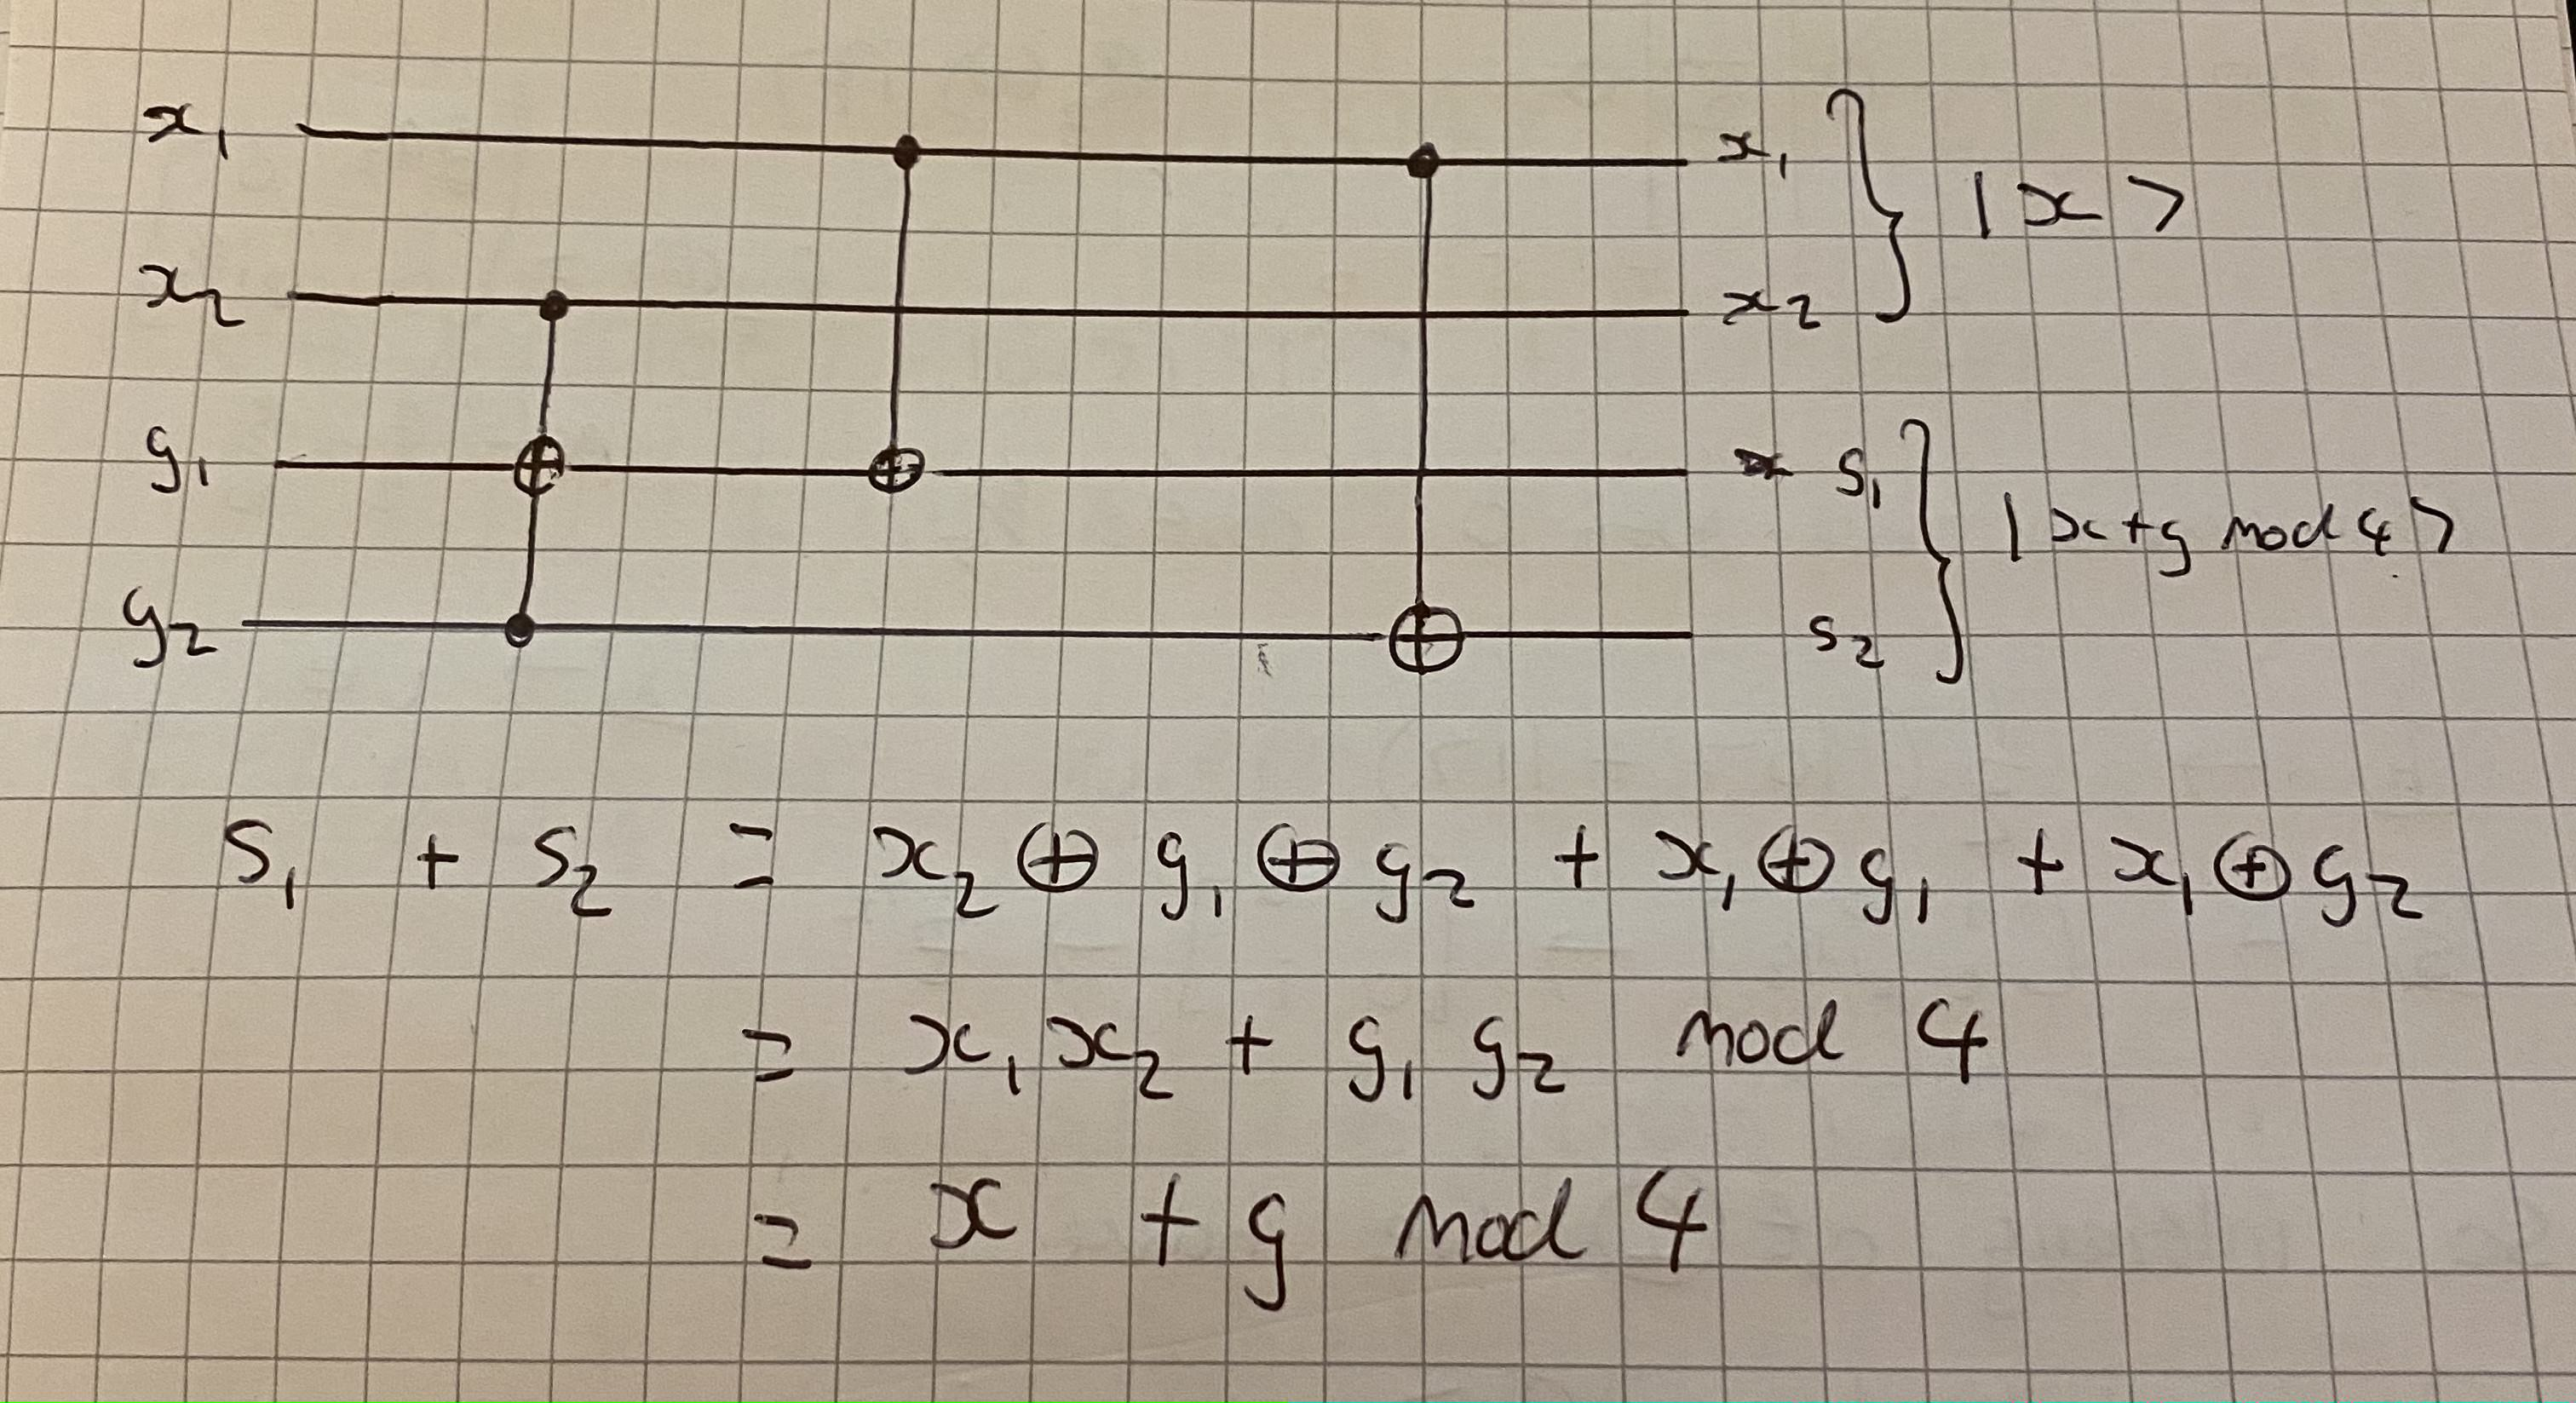
\includegraphics[width=8cm]{436.jpg}
    \centering
    \caption{Quantum circuit for Ex 4.36 to add two two-bit numbers mod 4. The text below the circuit verifies that the outputs combine to give $x+y \ mod \ 4$. This image is also attached separately.}
\end{figure}

\item \textbf{\underline{Exercise 4.42 from Nielsen \& Chuang.}} 
\\
Irrationality of $\theta$ with $cos(\theta) = 3/5$ 
\begin{enumerate}
    \item (1) 
    \\
    $$ e^{i \theta} = \frac{3+4i}{5} $$
    Because $\theta$ must be rational (as given in the question $\theta$ must be a multiple of $2\pi$) we can say that 
    $$ e^{im \theta} = e^{ik} = 1 $$
    Where $k= 2 \pi \theta$ so that 
    $$ e^{i m \theta} = \frac{(3+4i)^m}{5^m}$$
    $$ 1 \times 5^m = (3+4i)^m $$
    Such that we get that there must be a positive integer m such that 
    $$ (3 +4i)^m = 5^m$$ 

    \item (2) Showing that $(3+4i)^m = 3+4i (mod \ 5) $ for all $m > 0$ 
    \\
    So for $m=1$, trivially we have 
    $$ 3+4i = 3+4i \ mod \ 5 $$ 
    and for $m=2$ we have 
    $$ (3+4i)^2 = (3+4i)(3+4i) = 9 +12i +12i +16i^2 = -7 +24i = (3+4i) \ mod \ 5 $$ 
    It is (fairly?) safe to say that $m >0$ they're equal. This is saying that $3+4i$ is not a multiple of 5, therefore we can say 
    $$ 5^m = 0 \mod \ 5 $$ 
    So there cannot exist a $m$ which satisfies $(3+4i)^m = 5^m$
\end{enumerate}


\item \textbf{\underline{Exercise 4.51 from Nielsen \& Chuang.}}
\\
Construct a quantum circuit to simulate the Hamiltonian 
$$ H = X_1 \otimes Y_2 \otimes Z_3 $$ 
Performing $e^{-i \Delta t H}$ for any $\Delta t$ 
\\
Using Fig 4.19 in the book as a reference, we can transform the $X_1$ and $Y_1$ into Pauli $Z$ gates so the quantum circuit will be an alteration of fig 4.19. 
\\
The Pauli $X$ gate can be written as 
$$ X = HZH$$ 
As proved earlier in N \& C (eq 4.18). The Pauli $Y$ gate requires additional thought but it can be transformed into single qubit gate operations using equations 4.5 and 4.6 and exericse 4.7 in the book. 
\\
So the Pauli $Y$ gate can be decompised into the Pauli $X$ gate through applying a rotation matrix $R_z$ and then transforming the $X$ gate into a $Z$ gate through the equation above. (Similar to Toffoli gate transformation shown in Problem Set 6, which helped me in realising this.)
$$ R_z (\theta) =  \left(\begin{array}{cc} e^{-i \theta /2} & 0 \\  0 & e^{i \theta /2} \end{array}\right) $$
$$ R_z (-\theta) = \left(\begin{array}{cc} e^{i \theta /2} & 0 \\  0 & e^{-i \theta /2} \end{array}\right) $$
If we take $\theta = \frac{\pi}{2}$ we get back to $Y$ such that 
$$ Y = R_z (\theta) X R_z (-\theta) $$
Which, if we think about in terms of the bloch sphere representation intuitively makes sense with a rotation of 90 degrees, which is why $\theta = \frac{\pi}{2}$ was applied. 
$$  Y = R_z ( \frac{\pi}{2}) X R_z (- \frac{\pi}{2}) $$
$$ = \left(\begin{array}{cc} e^{-i \frac{\pi}{4}} & 0 \\  0 & e^{i \frac{\pi}{4}} \end{array}\right) \left(\begin{array}{cc} 0 & 1 \\  1 & 0 \end{array}\right) \left(\begin{array}{cc} e^{i \frac{\pi}{4}} & 0 \\  0 & e^{-i \frac{\pi}{4}} \end{array}\right) = \left(\begin{array}{cc} 0 & -i \\  i & 0 \end{array}\right) $$
Which, using $X = HZH$ makes this 
$$ Y = R_z (\frac{\pi}{2}) HZH R_z(- \frac{\pi}{2}) $$
Now both $X$ and $Y$ are written as single qubit gates to $Z$ operations, the Hamiltonians is 
$$ H = H_1 Z_1 H_1 \otimes R_{z_2}(\frac{\pi}{2}) H_2 Z_2 H_2 R_{z_2}(-\frac{\pi}{2}) \otimes Z_3 $$

\begin{figure}[h]
    
    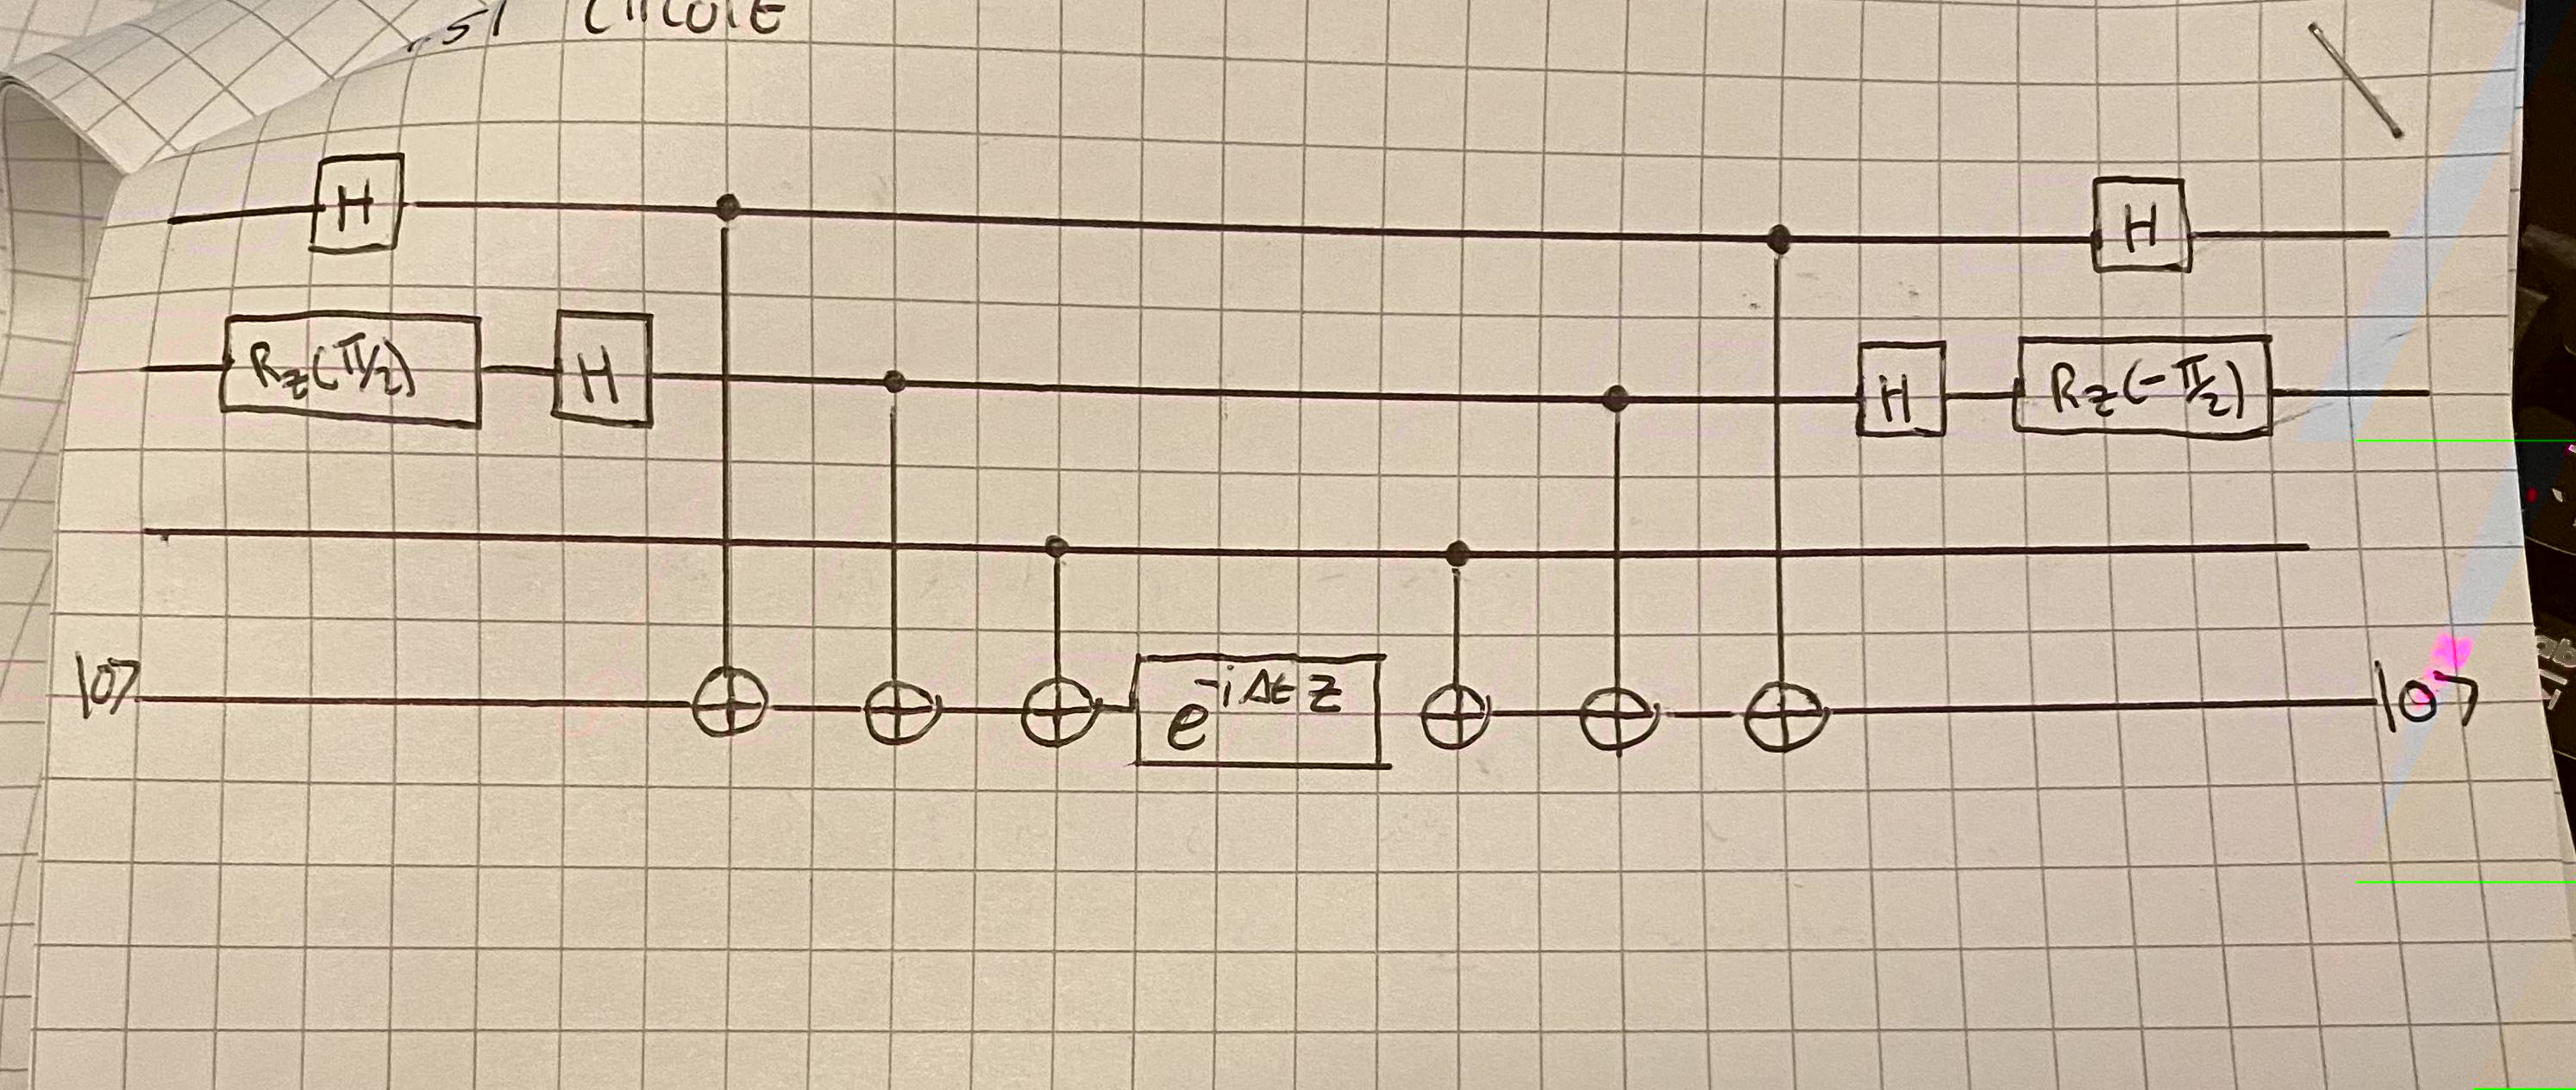
\includegraphics[width=8cm]{451.jpg}
    \centering
    \caption{Quantum circuit for Ex 4.51.This image is also attached separately.}
\end{figure}


\item \textbf{\underline{Exercise 5.18 from Nielsen \& Chuang.}}
\\
Factoring $N=91$. Following the algorithm for reduction of factoring to order finding. 
\\ 
Step 1: Is N even? No. \\
Step 2: Does $N=a^b$ for $a \geq 1$ and $b \geq 2$. Using a quick python check (not necessary but quick), the closest we get is $9^2 = 81$ or $3^4 = 81$. $N \neq a^b$ for integers $a$ and $b$. 
\\
Step 3: $x=4$
$$ gcd(x,N) = gcd(4,91) = 1$$
So step 3 is also skipped. 
\\
Step 4: Find order $r$ of $x \ mod \ 91$. Again using python 
$$ 4^1 = 4 \rightarrow 4 \ mod \ 91 =4 $$
$$ 4^2 = 16 \rightarrow 16 \ mod \ 91 =16 $$
$$ 4^3 = 64 \rightarrow 64 \ mod \ 91 =64 $$
$$ 4^4 = 256 \rightarrow 256 \ mod \ 91 =74 $$
$$ 4^5 = 1024 \rightarrow 1024 \ mod \ 91 =23 $$
$$ 4^6 = 4096 \rightarrow 4096 \ mod \ 91 =1 $$
So $r=6$ and $r$ is even so for Step 5 we have 
$$ 4^{\frac{r}{2}} = 4^3 = 64 \neq -1(mod \ 91) \neq 90 $$
And 
$$ gcd(64-1, 91) = 7 $$
And the algorithm succeeds.


\end{enumerate}


\end{document}

